\documentclass{article}
\usepackage{fullpage}
\usepackage{amsmath}
\usepackage{amsfonts}
\usepackage{authblk,caption}
\usepackage{titling}
\usepackage{tikz}
\usepackage{hyperref}
\usepackage{caption}
\usepackage{graphicx}
\graphicspath{{images/}}
\title{\huge{Classical Mechanics 1, Autumn 2021 CMI \\ Problem set 9\\\hspace{7cm}- Govind S. Krishnaswami}
}
\author{Soham Chatterjee\\Roll: BMC202175}
\date{}
\renewcommand\maketitlehooka{\null\mbox{}\vfill}
\renewcommand\maketitlehookd{\vfill\null}
\newcommand{\delx}{\Delta_x}
\newcommand{\delt}{\Delta_t}
\setlength{\parindent}{1cm}
\begin{document}
	%---------------------------------------
% BlackBoard Math Fonts :-
%---------------------------------------

%Captital Letters
\newcommand{\bbA}{\mathbb{A}}	\newcommand{\bbB}{\mathbb{B}}
\newcommand{\bbC}{\mathbb{C}}	\newcommand{\bbD}{\mathbb{D}}
\newcommand{\bbE}{\mathbb{E}}	\newcommand{\bbF}{\mathbb{F}}
\newcommand{\bbG}{\mathbb{G}}	\newcommand{\bbH}{\mathbb{H}}
\newcommand{\bbI}{\mathbb{I}}	\newcommand{\bbJ}{\mathbb{J}}
\newcommand{\bbK}{\mathbb{K}}	\newcommand{\bbL}{\mathbb{L}}
\newcommand{\bbM}{\mathbb{M}}	\newcommand{\bbN}{\mathbb{N}}
\newcommand{\bbO}{\mathbb{O}}	\newcommand{\bbP}{\mathbb{P}}
\newcommand{\bbQ}{\mathbb{Q}}	\newcommand{\bbR}{\mathbb{R}}
\newcommand{\bbS}{\mathbb{S}}	\newcommand{\bbT}{\mathbb{T}}
\newcommand{\bbU}{\mathbb{U}}	\newcommand{\bbV}{\mathbb{V}}
\newcommand{\bbW}{\mathbb{W}}	\newcommand{\bbX}{\mathbb{X}}
\newcommand{\bbY}{\mathbb{Y}}	\newcommand{\bbZ}{\mathbb{Z}}

%---------------------------------------
% MathCal Fonts :-
%---------------------------------------

%Captital Letters
\newcommand{\mcA}{\mathcal{A}}	\newcommand{\mcB}{\mathcal{B}}
\newcommand{\mcC}{\mathcal{C}}	\newcommand{\mcD}{\mathcal{D}}
\newcommand{\mcE}{\mathcal{E}}	\newcommand{\mcF}{\mathcal{F}}
\newcommand{\mcG}{\mathcal{G}}	\newcommand{\mcH}{\mathcal{H}}
\newcommand{\mcI}{\mathcal{I}}	\newcommand{\mcJ}{\mathcal{J}}
\newcommand{\mcK}{\mathcal{K}}	\newcommand{\mcL}{\mathcal{L}}
\newcommand{\mcM}{\mathcal{M}}	\newcommand{\mcN}{\mathcal{N}}
\newcommand{\mcO}{\mathcal{O}}	\newcommand{\mcP}{\mathcal{P}}
\newcommand{\mcQ}{\mathcal{Q}}	\newcommand{\mcR}{\mathcal{R}}
\newcommand{\mcS}{\mathcal{S}}	\newcommand{\mcT}{\mathcal{T}}
\newcommand{\mcU}{\mathcal{U}}	\newcommand{\mcV}{\mathcal{V}}
\newcommand{\mcW}{\mathcal{W}}	\newcommand{\mcX}{\mathcal{X}}
\newcommand{\mcY}{\mathcal{Y}}	\newcommand{\mcZ}{\mathcal{Z}}



%---------------------------------------
% Bold Math Fonts :-
%---------------------------------------

%Captital Letters
\newcommand{\bmA}{\boldsymbol{A}}	\newcommand{\bmB}{\boldsymbol{B}}
\newcommand{\bmC}{\boldsymbol{C}}	\newcommand{\bmD}{\boldsymbol{D}}
\newcommand{\bmE}{\boldsymbol{E}}	\newcommand{\bmF}{\boldsymbol{F}}
\newcommand{\bmG}{\boldsymbol{G}}	\newcommand{\bmH}{\boldsymbol{H}}
\newcommand{\bmI}{\boldsymbol{I}}	\newcommand{\bmJ}{\boldsymbol{J}}
\newcommand{\bmK}{\boldsymbol{K}}	\newcommand{\bmL}{\boldsymbol{L}}
\newcommand{\bmM}{\boldsymbol{M}}	\newcommand{\bmN}{\boldsymbol{N}}
\newcommand{\bmO}{\boldsymbol{O}}	\newcommand{\bmP}{\boldsymbol{P}}
\newcommand{\bmQ}{\boldsymbol{Q}}	\newcommand{\bmR}{\boldsymbol{R}}
\newcommand{\bmS}{\boldsymbol{S}}	\newcommand{\bmT}{\boldsymbol{T}}
\newcommand{\bmU}{\boldsymbol{U}}	\newcommand{\bmV}{\boldsymbol{V}}
\newcommand{\bmW}{\boldsymbol{W}}	\newcommand{\bmX}{\boldsymbol{X}}
\newcommand{\bmY}{\boldsymbol{Y}}	\newcommand{\bmZ}{\boldsymbol{Z}}
%Small Letters
\newcommand{\bma}{\boldsymbol{a}}	\newcommand{\bmb}{\boldsymbol{b}}
\newcommand{\bmc}{\boldsymbol{c}}	\newcommand{\bmd}{\boldsymbol{d}}
\newcommand{\bme}{\boldsymbol{e}}	\newcommand{\bmf}{\boldsymbol{f}}
\newcommand{\bmg}{\boldsymbol{g}}	\newcommand{\bmh}{\boldsymbol{h}}
\newcommand{\bmi}{\boldsymbol{i}}	\newcommand{\bmj}{\boldsymbol{j}}
\newcommand{\bmk}{\boldsymbol{k}}	\newcommand{\bml}{\boldsymbol{l}}
\newcommand{\bmm}{\boldsymbol{m}}	\newcommand{\bmn}{\boldsymbol{n}}
\newcommand{\bmo}{\boldsymbol{o}}	\newcommand{\bmp}{\boldsymbol{p}}
\newcommand{\bmq}{\boldsymbol{q}}	\newcommand{\bmr}{\boldsymbol{r}}
\newcommand{\bms}{\boldsymbol{s}}	\newcommand{\bmt}{\boldsymbol{t}}
\newcommand{\bmu}{\boldsymbol{u}}	\newcommand{\bmv}{\boldsymbol{v}}
\newcommand{\bmw}{\boldsymbol{w}}	\newcommand{\bmx}{\boldsymbol{x}}
\newcommand{\bmy}{\boldsymbol{y}}	\newcommand{\bmz}{\boldsymbol{z}}
	
	\maketitle\pagebreak
	
	\begin{enumerate}
		\item The frame $S'$ that coincides with frame $S$ at $t = t' = 0$ and moves uniformly at speed $v$ along the positive $x$ axis of $S$. Hence $$x'=\gamma(x-vt)\qquad \text{and}\qquad  t'=\gamma\left(t-\frac{vx}{c^2}\right)$$Hence $$x_2'-x_1'=\gamma((x_2-x_1)-v(t_2-t_1))\qquad\text{and}\qquad t_2'-t_1'=\gamma\left((t_2-t_1)-\frac{v(x_2-x_1)}{c^2}\right)$$Let's denote $\delx=x_2-x_1$ and $\delt=t_2-t_1$. Hence given that $c^2\delt^2-\delx^2=\Delta$ Now\begin{align*}
			c^2(t_2'-t_1')^2-(x_2'-x_1')^2\ &=c^2\gamma^2\left(\delt-\frac{v\delx}{c^2} \right)^2- \gamma^2(\delx-v\delt)^2\\
			&=\gamma^2\Bigg[\left(c\delt-\frac{v\delx}{c} \right)^2- (\delx-v\delt)^2\Bigg]\\
			&=\gamma^2\Bigg[\left( c^2\delt^2+\frac{v^2\delx^2}{c^2}-2v\delt\delx\right) -(\delx^2+v^2\delt^2-2v\delx\delt)\Bigg]\\
			&=\gamma^2\Bigg[\delt^2\left(c^2-v^2 \right)-\delx^2\left(\frac{v^2}{c^2}-1\right) \Bigg]\\
			&=c^2\delt^2-\delx^2=\Delta
		\end{align*}
		Hence the square of space-time separation is unchanged under Lorentz Transformation.
		\item \begin{enumerate}
			\item \begin{align*}
				E^2-\bmp^2c^2 \ & =\gamma^2  m^2c^4-\gamma^2m^2\bmv^2c^2 \\
				                & =\gamma^2m^2c^2(c^2-\bmv^2)\\
				                & =m^2c^4=(mc^2)^2
			\end{align*}
			\item \begin{align*}
				\gamma \ &=\left(1-\frac{\bmv^2}{c^2} \right)^{\frac12}\approx1+\frac12\frac{\bmv^2}{c^2}
			\end{align*}Here wr are ignoring the higher order terms of $\frac{\bmv^2}{c^2}$ for non-relativistic limit. Hence\begin{align*}
			&E=\gamma mc^2\approx mc^2\left(1+\frac{\bmv^2}{2c^2}\right)=mc^2+\frac{m\bmv^2}{2}\\
			&\bmp=\gamma m\bmv\approx m\bmv\left(1+\frac{\bmv^2}{2c^2}\right)=m\bmv +\frac{m\bmv^3}{2c^2}
		\end{align*}
			\item According to the dispersion relation $E^2-\bmp^2c^2=(mc^2)^2\implies E^2=(mc^2)^2+\bmp^2c^2$. Hence\begin{align*}
				E\ & =\left((mc^2)^2+\bmp^2c^2\right)^{\frac12}                \\
				   & =mc^2\left(1+\frac{\bmp^2c^2}{m^2c^4}\right)^{\frac12}    \\
				   & =mc^2\left(1+\frac{\bmp^2}{m^2c^2}\right)^{\frac12}       \\
				   & \approx mc^2\left(1+\frac12\,\frac{\bmp^2}{m^2c^2}\right) \\
				   & =mc^2+\frac{\bmp^2}{2m}
			\end{align*}
		\end{enumerate}
	
	\item \begin{enumerate}
		\item In the graph we have taken $E$ in the $x$-axis, $p_1$ in the $y$-axis and $p_2$ in the $z$-axis.
		
		\begin{figure}[h]
			\centering
			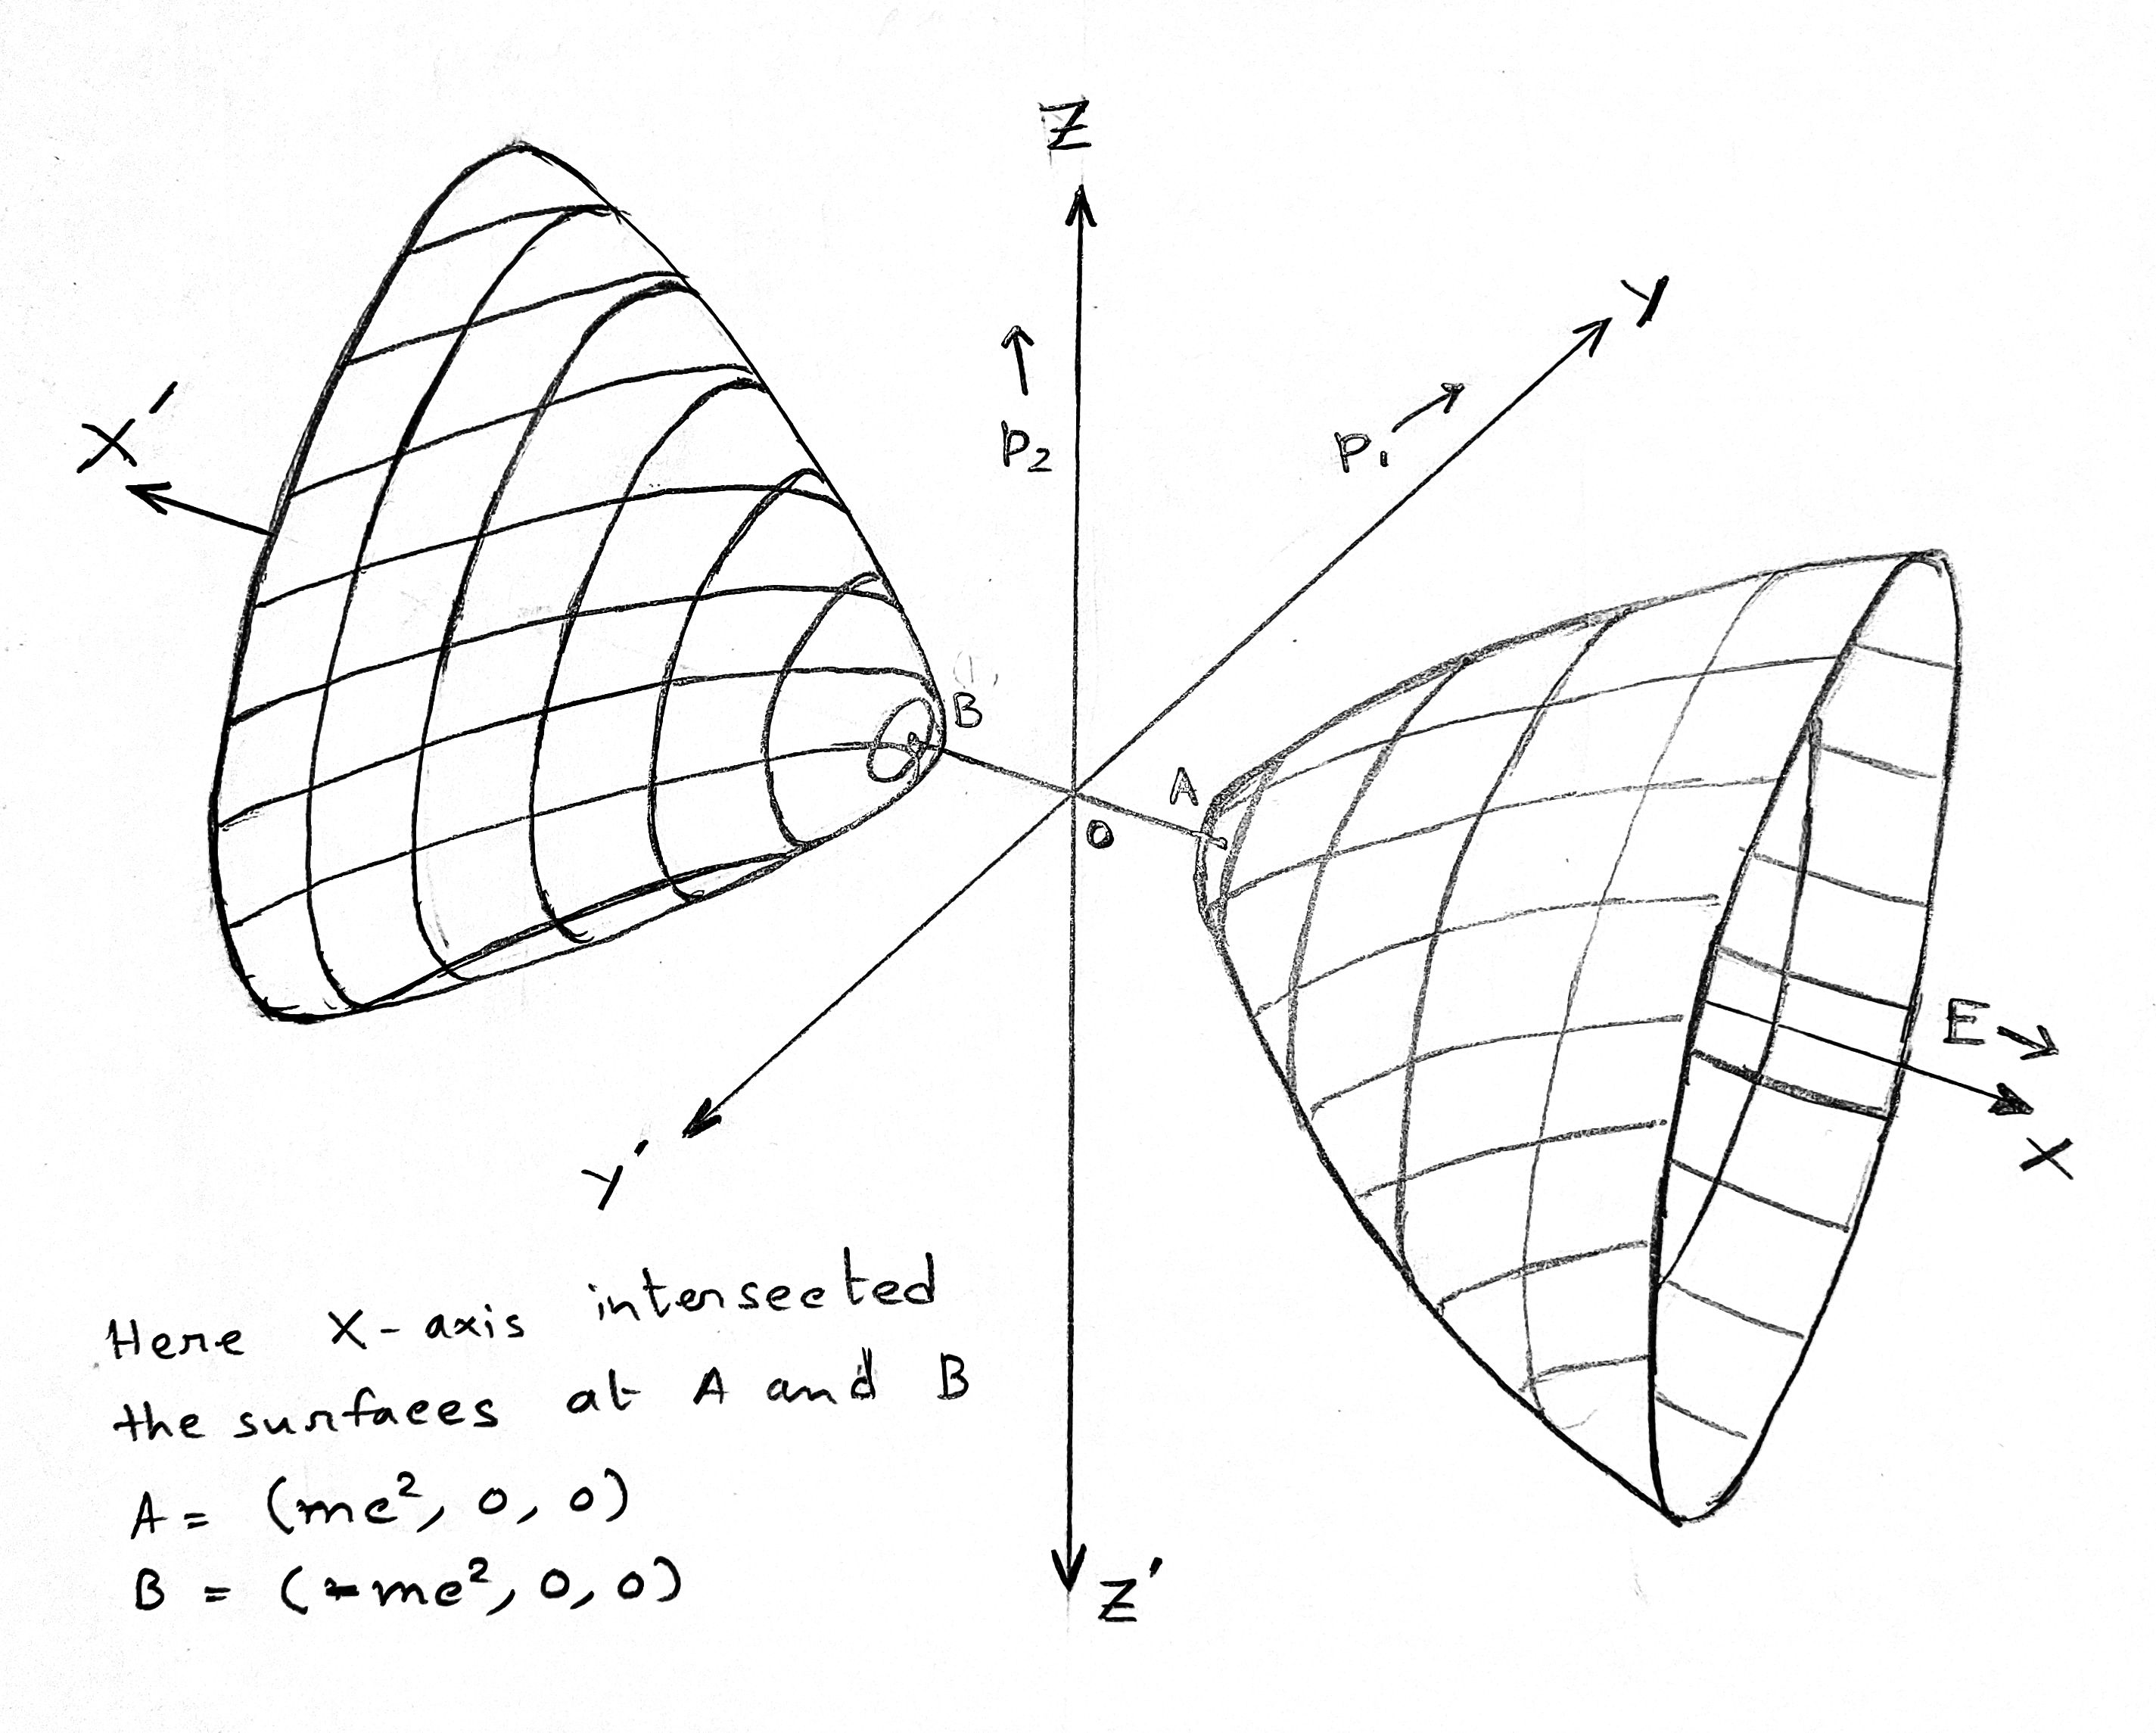
\includegraphics[width=14cm]{2.jpg}
			\caption*{Figure: Surface of $E-p_1-p_2$ in $\bbR^3$}
			\end{figure}Here the $x$-axis intersected the surfaces in two points. It intersected in positive side at $(mc^2,0,0)$ and in negative side at $(-mc^2,0,0)$
		\item Name of the surface can be ``Relativistic Dispersion Surface''
		\item Since $E=\gamma mc^2$ we can say $E>0$. Hence the surface which is in the negative side of the $x$-axis is not physically relevant There fore the surface in the positive direction of $x$-axis is physically relevant.
	\end{enumerate}
	\item \begin{enumerate}
		\item I select the chapters \begin{itemize}
			\item Collisions or scattering and conservation laws
			\item Special theory of relativity
		\end{itemize}
	\item Let we have two identical rods $l_1,l_2$  of length $l$ and mass $m$ (The rods have uniform mass distribution. Hence the centre of the rods are centre of mass). Suppose $l_1$ is in rest along the $x$ axis whose left end is at the $\left(\frac{l}{2},0\right)$. $l_2$ parallel to $x$-axis and it is approaching towards the origin from the positive side of $y$-axis with velocity $v$ whose centre is on the $y$-axis such that it collides with $l_1$ at the end point.
	\begin{itemize}
		\item After the collision the rods will start rotating about their centres. As $l_2$'s right end collided with $l_1$'s left end  both $l_1$ and $l_2$ will start rotating counter-clockwise if we observe from the positive direction of $z$-axis. See here before the collision their was no angular momentum . But after the collision they have angular momentum which does not cancel out each other instead add up. Hence angular momentum conservation rule didn't follow here. But as per the law in absence of torque angular momentum is supposed to be conserved. What exactly wrong here ?
		\item If we know $m,l,v$ then the whole situation after the collision is predetermined. How to calculate the final outcome in general condition ?
	\end{itemize}
	\item Suppose $S$ is an inertial frame. $S'$ is a frame which moving at the speed of light $c$ relative to $S$. Then $\gamma$ becomes infinite. Hence with respect to $S$ any time interval in $S$ becomes 0 in $S'$. Hence everything in $S$ happens instantaneously in $S'$. In that case any time interval in $S'$ makes no sense. Then how can we apply Lorentz Transformation here where in one frame time interval does not make sense and in another frame time interval makes sense. If time interval does not make sense in $S'$ how can we define time in $S'$ ?
	\end{enumerate}
	\end{enumerate}
	
\end{document}